%!TEX root = ../PhDthesis.tex
\chapter{Long-range interactions in the visual cortex}

One of the most striking features in the early visual cortex is the
presence of patchy long-range excitatory connections linking regions
with similar feature preferences. These connections have been
suggested to drive a wide range of contextual modulation effects
including pop-out, iso-orientation suppression, contour completion and
more \citep{Gilbert1983, Hirsch1991, McGuire1991, Grinvald1994,
  Fitzpatrick2000, Hupe2001, Stettler2002}. Even though these
connections are excitatory it is now well established that they also
provide inhibition via a di- or poly-synaptic mechanism
\citep{Weliky1995}. While both the SCAL and SEPI models optionally
have long-range excitation these connections, since these connections
are purely excitatory they cannot mediate long-range suppressive
effects directly and due to the weakly tuned nature of the PV cell
population they too are not viable candidates to mediate feature
specific contextual modulation effects such as iso-orientation
suppression.

A major feature of the neural code in the cortex is the elimination of
redundancy in order to achieve a sparse representation of the input
\citep{Olshausen1996}. Indeed it has been found that modulation from
the nonclassical receptive field suppresses redundant information in
the input sparsifying the neural code \citep{Vinje2000}. In previous
developmental models of the primary visual cortex it was shown that
allowing lateral inhibitory connections to develop non-isotropic
connectivity, which allows the network to learn the redundant features
of the input and suppress them, results in a sparser representation
\citep{Miikkulainen2005b}. If such development is not allowed to take
place and isotropic surround suppression is employed,
cross-orientation stimuli, belonging to a separate object or contour
may be suppressed, thus reducing the information content encoded by
the network.

This suggests a difference between short scale interactions where the
cortex is trying to ensure it achieves maximal coverage of the feature
space and long-range interactions where the neuron is competing to
represent the stimulus itself in an efficient way, i.e. by using a
sparse code. In the previous models the PV inhibition drove the local
competition resulting in a smooth coverage of the visual space with
orientation feature detectors, i.e. an orientation map. Since these
neurons act over a fairly small range and are not highly tuned in the
orientation domain they are generally isotropic in the spatial
distribution and cannot mediate feature specific modulation.

In the literature we have identified a second population of inhibitory
interneurons with interesting properties. The Somatostatin
immunoreactive (Sst) neurons are the second largest group of
interneurons \citep{Gonchar2007,Xu2010} and exhibit very different
properties from the PV population, which makes them interesting as a
candidate to perform long-range integration of inputs. Specifically
they are enriched in layer 2/3 where a lot of the long-range patchy
connectivity is found and they seem to respond strongly only under
strong, sustained stimulation \citep{Ma2011} or for very large stimuli
\citep{Adesnik2012}. Additionally the input scaling does not seem to
be linear, with a accelerating response function driving much stronger
responses when they recruited consistently and robustly (as would be
the case for large or high contrast stimuli)
\citep{Beierlein2003,Bartley2008,Tan2008}.

On the basis of what we have learned about the PV population from the
previous models and what we know about Somatostatin neurons from the
literature we therefore propose a general theory of how the circuit
performs specific computations. Afferent input provides strong,
low-latency excitation to the Pv-ir neurons in the thalamocortical
recipient layer 4, which in turn act as both a feedforward inhibition
and dynamic gain control mechanism on the broadly activated excitatory
cell population. This results in local decorrelation of the neural
activity, which allows recurrent excitation to amplify the activity in
the local neural ensemble, which leads to the formation of a smooth
orientation map.

At the same time Sst-ir neurons begin to integrate the local activity
through the local and long-range orientation-specific lateral
connections. If their inputs are sufficiently strong they will
activate strongly allowing this polysynaptic circuit to reduce
long-range correlation in the input activity, further reducing
redundancy. If they are only weakly activated, as would occur when
presented with low-contrast or very sparse input patterns, long-range
lateral excitatory connections are not outcompeted and the circuit can
fill in weak or missing information based on past statistics. In such
a regime the differential recruitment of the two separate inhibitory
populations would be responsible for a shift in cortical state from a
mode of redundancy-reduction and feature discrimination to one of
visual inference.

In this chapter we further extend the existing SEPI model by adding
this second population of inhibitory neurons modelled after the Sst
interneuron population. In doing so we will demonstrate how this
second population integrates large and high-contrast stimuli providing
feature specific inhibition under those conditions, while only very
weakly responding in low contrast conditions. This provides a
considerable advance over previous models, which differ in that they
usually hard-code the statistical relationships encoded in the lateral
connections and generally explain contrast dependent changes through a
higher inhibitory threshold, which is generally not supported by
evidence. The contextual modulation effects are therefore an emergent
phenomenon, arising from the correlations present in the training
patterns. Identifying and modeling the circuits involved in these
processes is a fundamental challenge for neuroscience and will hugely
contribute to extending our understanding of cortical information
processing.

\section{Methods}

\subsection{The LESPI model}

The \textbf{L}ong-\textbf{R}ange \textbf{E}xcitation, \textbf{S}sst
and \textbf{PV} \textbf{I}nhibition (LESPI) model again builds on the
previous models introducing an additional population of inhibitory
neurons, which is entirely recurrently driven via short- and
long-range projections by the two other populations. The diagram in
\ref{LESPIDiagram} shows how the three populations of V1 neurons are
recurrently connected.

The newly introduced Sst population will differ from the PV population
in a number of respects. First of all it receives no afferent input
from the LGN, as this population is thought to be enriched in
supra-granular layers, which do not receive direct afferent
input. Secondly this population has a much more restricted spatial
profile being not nearly as extensive in their lateral extent as the
PV expressing basket cells. Most importantly however the facilitating
response properties of lateral synaptic connections contacting this
population is modeled via an exponential non-linearity in their
response. This allows this population to activate weakly in
low-contrast conditions, while providing strong suppression when the
input is strong or dense enough. Finally to model the more sluggish
responses among this population a hysteresis term is added. In this
way this population responds strongly after sustained and strong local
and long-range stimulation.

\subsubsection{Excitatory Activation}

The influence of the aggregate long-range excitatory and di-synaptic
inhibition via the Sst population is expressed as an additional
multiplicative factor modulating the response of the excitatory
neurons. The response of the excitatory population is then given by:

\begin{equation}
  \eta_{exc} = \frac{\eta_{A} + \eta_{LOC-EXC}}{1 + \eta_{PV-INH}} \eta_{SM}
\end{equation}

where $\eta_{A}$ is the LGN afferent activity, $\eta_{LOC-EXC}$ the local
excitatory contribution, $\eta_{PV-INH}$ the PV inhibitory contribution
and the surround modulation term $\eta_{SM}$ is defined as:

\begin{equation}
  \eta_{SM} = 1 + \eta_{LAT-EXC} - \eta_{Sst}
\end{equation}

where $\eta_{LAT-EXC}$ represents the long-range lateral excitatory
contribution and $\eta_{Sst}$ is the Sst inhibitory contribution. In
the SEPI model the $\eta_{SM}$ term simply reduces to 1, eliminating
all long-range interactions. The surround modulation term provides
gain when excitation exceeds inhibition and shunting inhibition when
the reverse is true. As such, this term provides a convenient
abstraction to model the modulatory influence of the dendritic
integration of long-range inputs, although in reality they will
provide both multiplicative/divisive and additive/subtractive effects.

\subsubsection{Inhibitory Sst Activation}

The activation of the inhibitory Sst population is given simply by the
summation of the local and lateral excitatory projection activity:

\begin{equation}
  \eta_{Sst} = \eta_{LOC-EXC} + \eta_{LAT-EXC}
\end{equation}

Additionally the $\eta_{LAT-EXC}$ term has an exponential activation
function applied to it such that it's contribution is given by

\subsubsection{Mechanisms}

The effective excitatory gain may not be a bad approximation to the
effect of long-range horizontal connections, which have been shown to
be strongly voltage dependent \citep{Hirsch1991}. Since Sst neurons
generally target distal dendrites they have generally been associated
with subtractive inhibition, they do however also have a
multiplicative component \citep{Wilson2012}. Additionally, their
preference for targetting distal dendrites may allow them to
effectively gate horizontal excitatory and feedback inputs
\citep{Ma2011, Gentet2012}. Additionally theoretical studies indicate
active dendritic spike backpropagation can lead to multiplicative
increases in gain, while reduction in spike backpropagation can lead
to divisive scaling of the firing rate \citep{Mehaffey2005}.

\begin{figure}
	\centering
        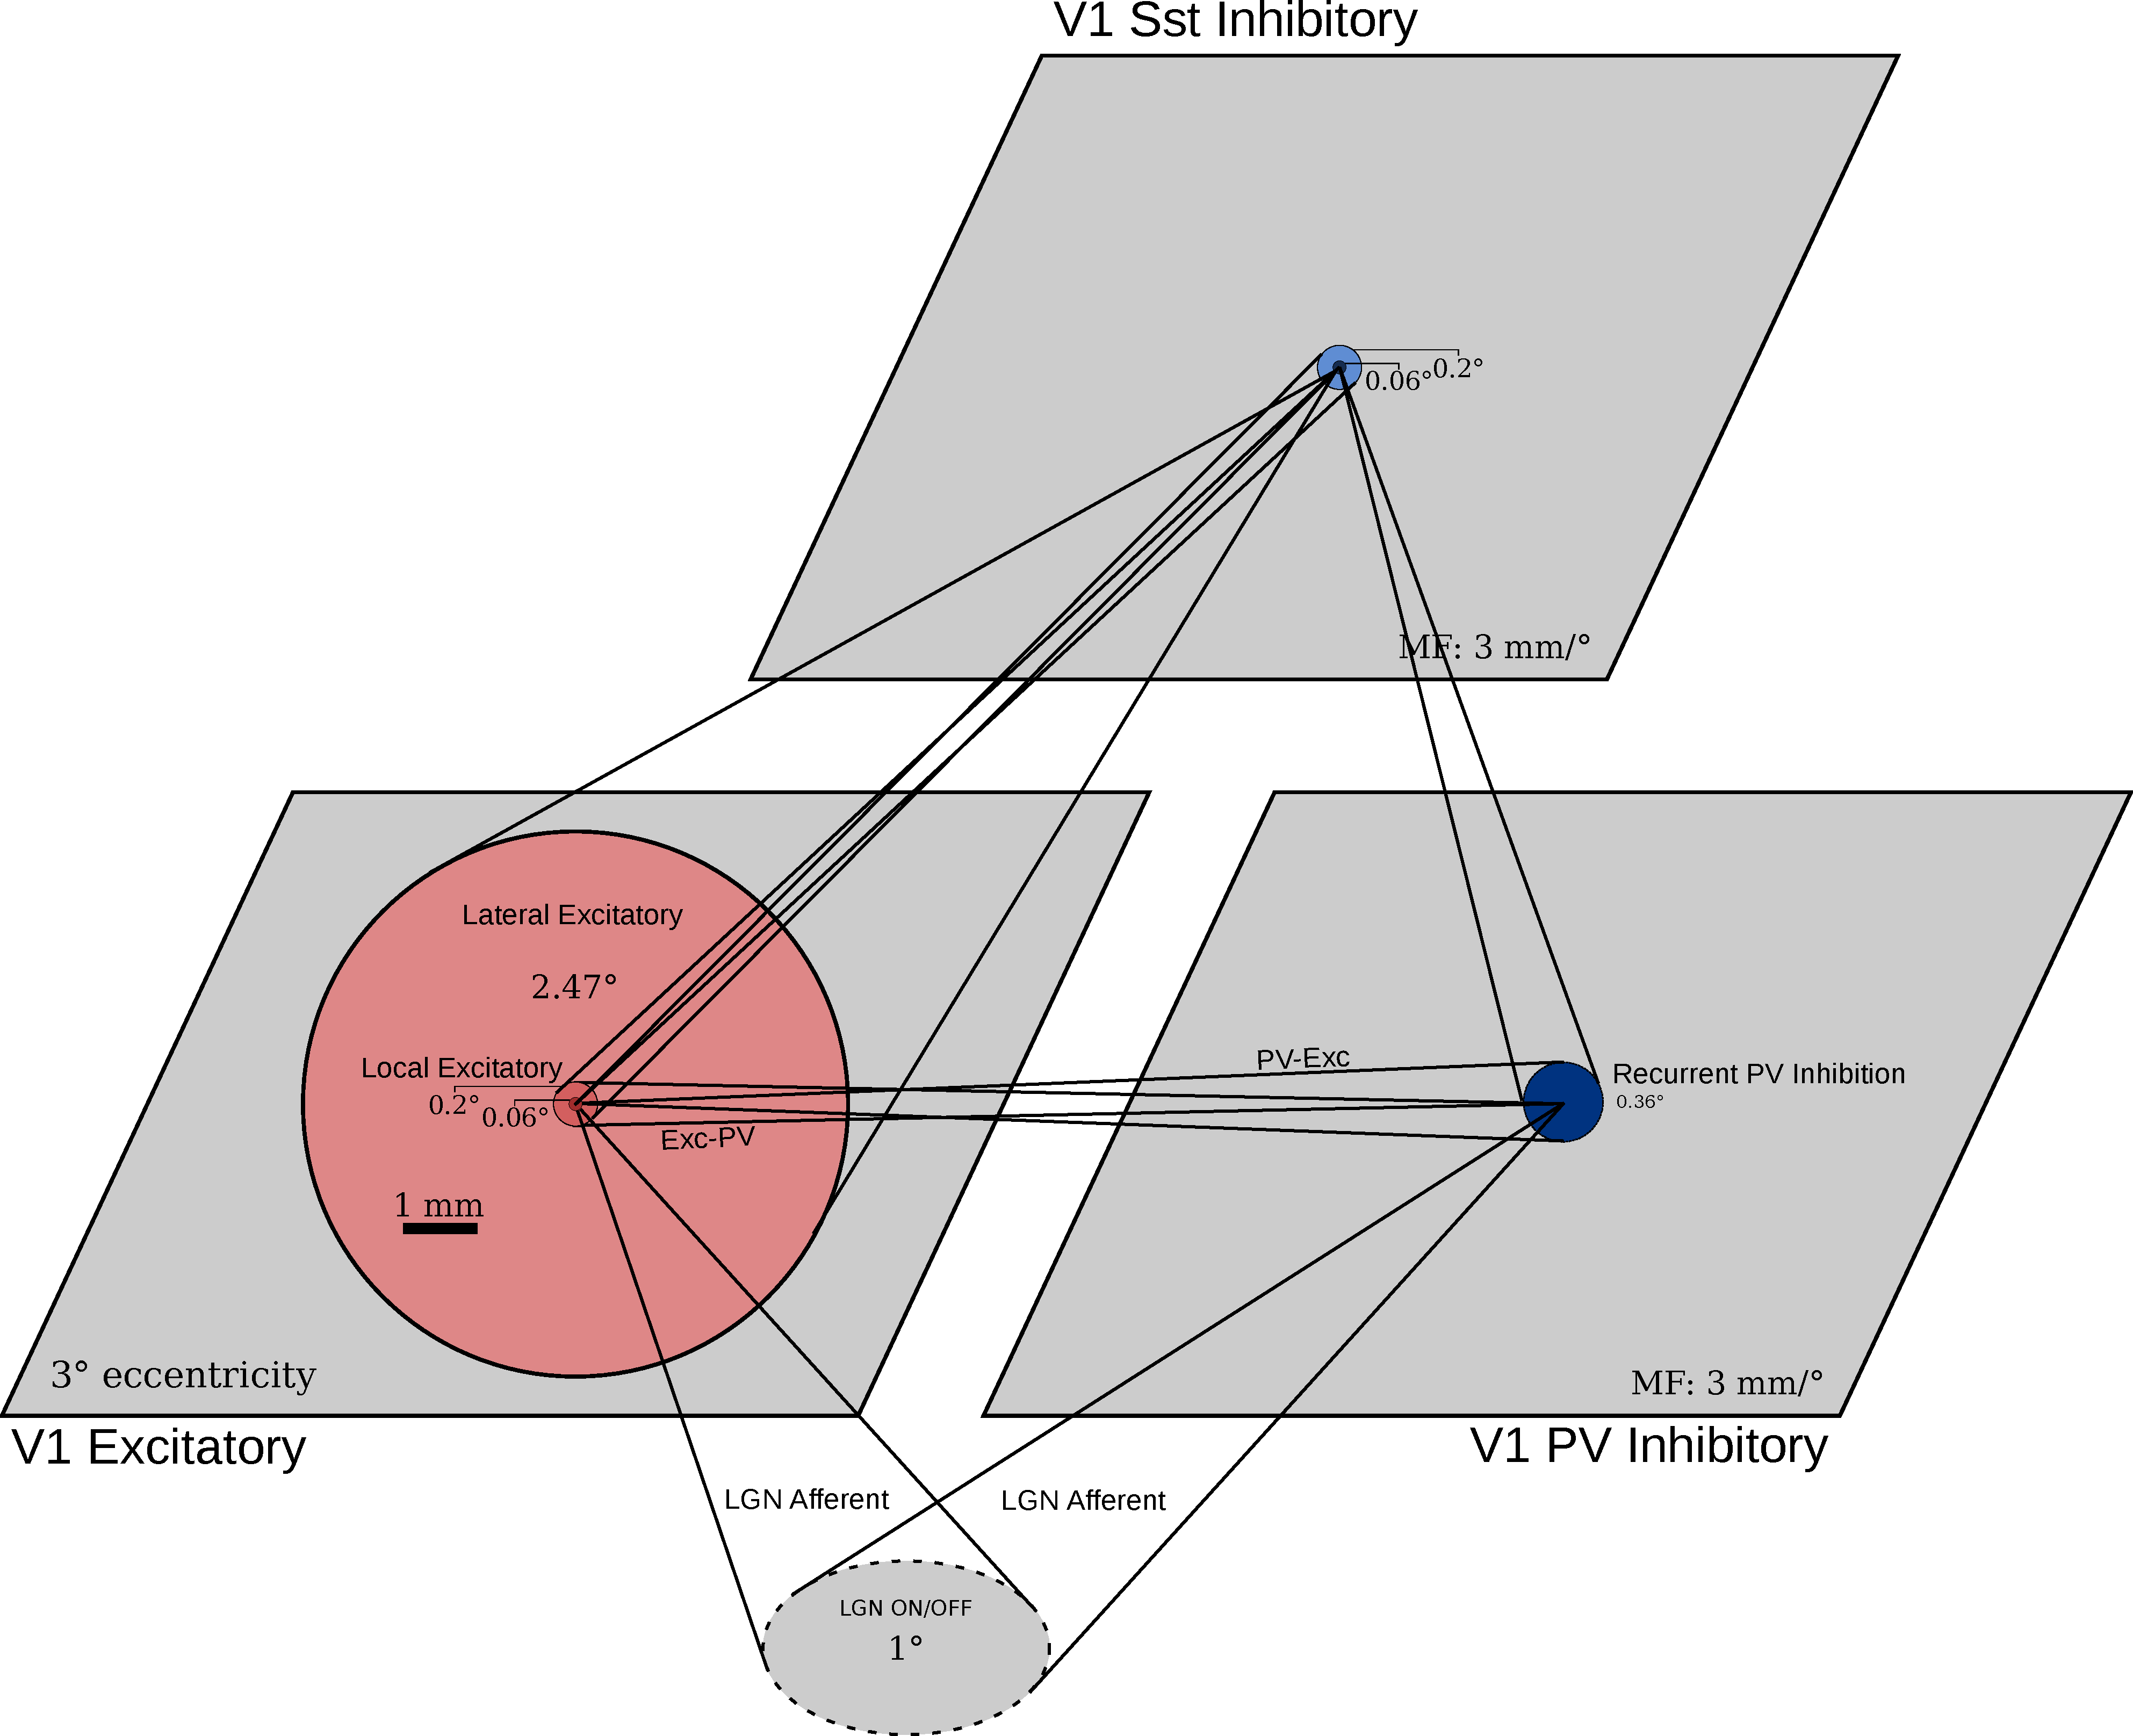
\includegraphics[width=1.0\textwidth]{LESPI_Diagram.pdf}
	\caption{Diagram of the LESPI V1 stage of the model showing the
          spatial scales of the various excitatory (red) and
          inhibitory (blue) connections. Satured colors indicate the
          kernel radii, while lightly shaded regions indicate kernel
          cut-off extents.}
	\label{LESPIDiagram}
\end{figure}

The overall operation of this circuit can be summarized by the
schematic in \ref{circuit_diagram}. The diagram shows the preferential
linking of columns with similar orientation preference via patchy
long-range connections and the long-range integration of Sst neurons,
which receive both local and lateral input from pyramidal neurons,
providing di-synaptic inhibition to the local region. Furthermore it
suggests that under low-contrast conditions the Sst population is
effectively disabled, activating only under high contrast input.

\begin{figure}
	\centering
	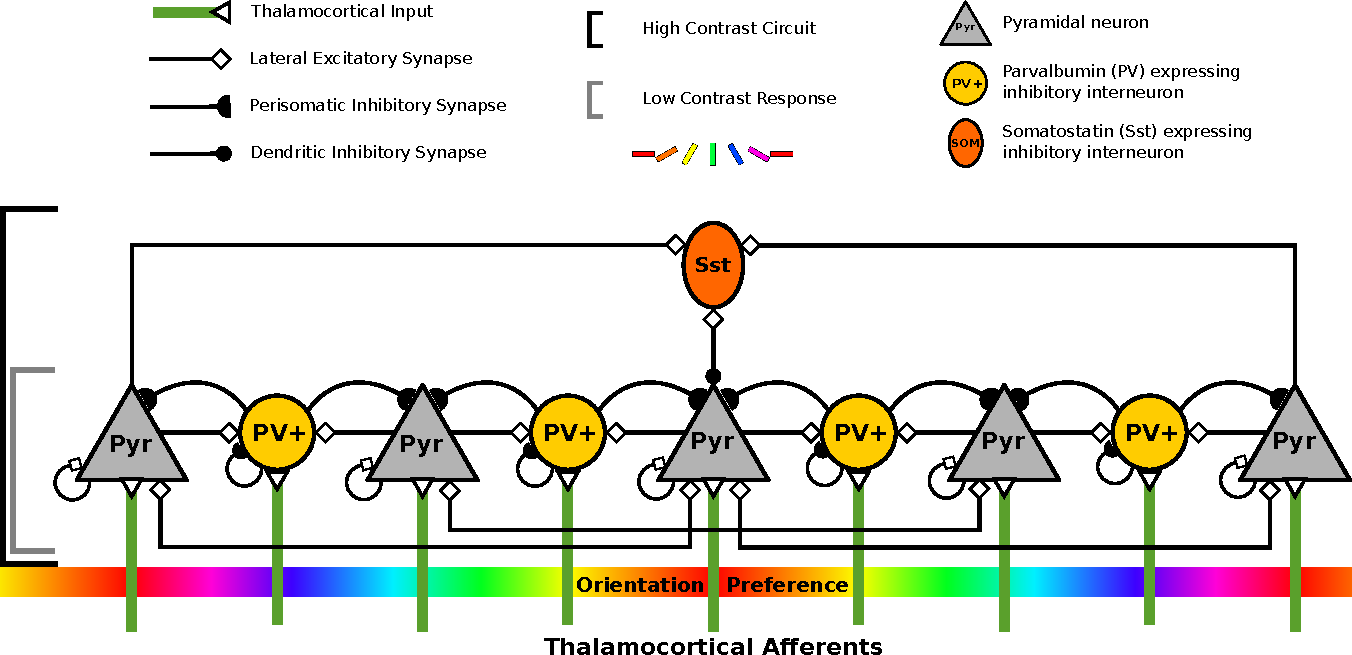
\includegraphics[width=1.0\textwidth]{./v1circuit.pdf}
	\caption[High-level circuit diagram of the LESPI
      model.]{High-level circuit diagram of the LESPI model. The
      schematic represents multiple hypercolumns varying smoothly in
      their orientation preference. PV neurons provide feedforward and
      recurrent inhibition to neurons to columns in the local region,
      regardless of their orientation tuning. Long-range excitatory
      connections link pyramidal cells with similar orientation
      preference, while the Sst population integrates both local and
      long-range input to provide tuned orientation suppression under
      high contrast input.}
    \label{circuit_diagram}
\end{figure}

\subsubsection{Sparsity}

In the current form of the model both afferent and lateral connection
fields are simulated as dense projections of weights in a local
region. However in reality lateral connections only form patchy
connections in the cortex. Having these diffuse connections means that
only a fraction of the synaptic weight is concentrated at the patchy
terminals. Informally we have confirmed that the model self-organizes
using a sparse sprouting and retraction algorithm, however this
sparsification algorithm should be validated separately before being
applied to the model, therefore the model is trained with dense
projections and are sparsified by thresholding the weights at the 90th
percentile. This leaves only patchy connections strongly resembling
experimental plots of patchy long-range connections in layer 2/3 of
macaque, extending up to 4 hypercolumns from neuron.

\subsection{Visual statistics}

So far we have mostly ignored the effect of visual statistics on the
model. This is in large part because the current model is based on
simple cells, which exhibit strong phase tuning, which is
unproblematic when trained on simple Gaussian stimuli but can lead to
disruptions in the map when both ON and OFF edges are present in the
visual inputs. However since the lateral connections in the model are
learned via Hebbian mechanisms the lack of long-range correlations
will be reflected in them, resulting in a lack of patchy connections
beyond the receptive field of the neuron. Therefore to observe any
real contextual modulation effects the visual input patterns need to
exhibit at least some long-range correlations. Therefore we will use a
number of different natural image datasets and synthetic Gaussian
stimuli with explicit long-range range correlations.

\subsubsection{Natural stimuli}

The visual statistics in natural stimuli can vary considerably, in
particular man-made objects often have very different statistics from
natural objects. This is because visual scenes in nature are dominated
by more circular contours while man-made objects usually exhibit more
straight and perpendicular lines. A range of experiments have shown
that humans can rapidly classify images of animals and non-animals
based solely on the co-occurence statistics of visual contours in the
image \citep{Serre2007, Perrinet2015}. Therefore we will make use of
the various image datasets used in these models to train the model on,
allowing us to compare the effect on contextual modulation.

The image datasets used for these purposes include the two target and
distractor dataset used by \cite{Serre2007} as well as multiple
datasets obtained by James Bednar meant to replicate the visual
experience of an animal both a laboratory environment, dominated by
high-contrast bars of the animal cages, and images of a natural
environment dominated mostly by trees, grass and leafs.

\begin{figure}
	\centering
	\includegraphics[width=1.0\textwidth]{./results/lespi/ImagePatterns.pdf}
	\caption[Example image patterns used to train the model] {Example
      image patterns sampled from different image datasets and then
      randomly positioned and rotated. A) Forest and grass taken in
      Gif-sur-Yvette B) Inside of a treeshrew cage taken in David
      Fitzpatrick lab C) \cite{Serre07} target patterns of animals and
      natural landscapes D) \cite{Serre07} distractor patterns of
      natural and man-made objects E) Inside ferret cages taken in
      David Fitzpatrick lab.}
    \label{image_patterns}
\end{figure}

\subsection{Surround modulation}

Beyond measuring simple attributes of the spatial organization in LGN
and V1, higher order effecs can be explored through complex surround
modulation measurement protocols. In addition to the simple area
summation curve measurements described above we replicate two further
protocols to evaluate the spatial response properties of the model.
In particular we are interested in the interaction between the spatial
arrangement of visual patterns presented to an animal and the contrast
on the response properties of visually responding neurons. For that
purpose we replicate two measurement protocols, a simple annulus based
contrast suppression measurement \cite{Jones2002} and a protocol using
target and flanker stimuli performed by \cite{Kapadia1995}.

\paragraph{Orientation contrast suppression}

The orientation contrast suppression is perhaps one of the most well
studied surround modulation paradigms. The measurement involves
presenting stimuli of a central sine grating, optimized to the
preferred size, frequency and orientation of the neuron being
measured. Once the baseline activity has been measured an additional
surround anulus with the same frequency is added and varied in
contrast, size and orientation to measure orientation dependent
interactions between center and surround (as shown in Figure
\ref{ORC_Stimulus}). In in-vivo experiments this measurements is
performed using drifting gratings with varying phase, since we are
only simulating simple cells the gratings are optimized for the
preferred phase of each neuron instead.

The center stimulus and the annulus were separated by $0.25^\circ$,
which is smaller than the size of the separation employed by
\cite{Jones2002}, however the size of the center and surround stimuli
were roughly the same scale with a $1^\circ$ and $3.5^\circ$ diameter
respectively.

\begin{figure}
	\centering
        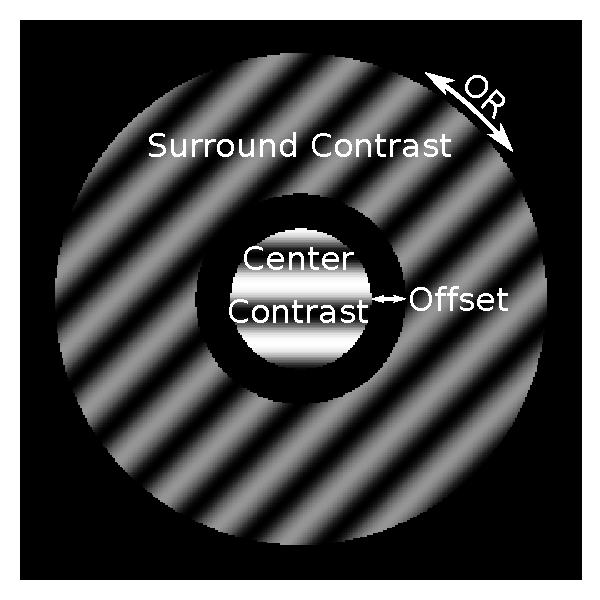
\includegraphics[width=0.5\textwidth]{ORC_Stimulus.pdf}
	\caption{Orientation contrast stimulus measuring modulation by a
      sine grating annulus on the response of a central neuron
      responding to a central sine grating disk of the same frequency.
      Stimulus is varied by center and surround contrast, surround
      orientation and the offset between the central disk and the
      surround annulus.}
	\label{ORC_Stimulus}
\end{figure}

The surround facilitation is quantified as:

\begin{equation}
F = (\frac{R_{cs}}{R_c} - 1) 100
\end{equation}

where $R_{CS}$ is the response of the combined stimulus and $R_C$ the
response to just the center stimulus.

\paragraph{Flanker Modulation}

Instead of working solely using area based protocols we also make use
of a simple bar based stimulus along with a flanker, which is
modulated in a number of ways to characterize the surround modulation
effects associated with this protocol. \cite{Kapadia1995} describe
a high degree of variability ranging from a complete lack of surround
modulation to facilitation and suppression. The three stimulus
protocols employed here are shown in \ref{Flanker}, we replicate these
protocol on the model to compare the effects observed in experiments
qualitatively.

\begin{figure}
	\centering
        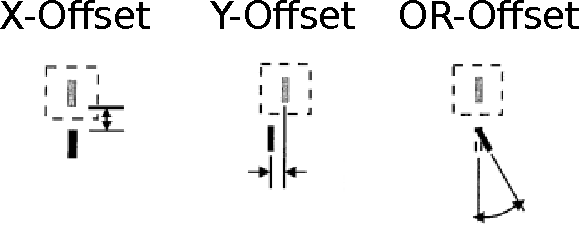
\includegraphics[width=1.0\textwidth]{FlankerProtocol.pdf}
	\caption[Flanker offset stimuli. Reproduced from
      \cite{Kapadia1995}.]{Flanker offset surround modulation
      paradigm. Measuring the effect of a flanker stimulus varying by
      an offset in X, Y and orientation on the response of a neuron to
      a target stimulus. Reproduced from \cite{Kapadia1995}.}
	\label{Flanker}
\end{figure}

\paragraph{Pop-out}

One of the most well studied effects in the surround modulation
literature is the pop-out effect, where when a visual stimulus is
embedded within a number of dissimilar features it strongly stands
out. It is thought this effect relies on similar features suppressing
each other leaving the dissimilar unaffected and therefore
``popping-out`` of the background \citep{Kastner1997}. In order to
test this surround modulation effect we generate visual patterns
container a target bar stimulus surrounded by a circle of flanker
stimuli, which are either co-aligned with the target (iso-condition)
or orthogonal to the target (cross-condition).

The response to the targets and the flankers is then computed as the
mean activity of the non-zero responding units with two annuli one
covering the central 1 degrees and the other covering the remaining
simulated area.

\section{Results}

As previously discussed the surround modulation effects in the model
are highly dependent on the statistics of the visual input the model
was trained on. Since the standard Gaussian patterns used so far do
not exhibit any long-range correlations the analyses here will use
models trained on natural images, which itself has some drawbacks,
however it allows the model to learn the statistics of the natural
world or of various laboratory environments. The following analyses
all use either the ``natural`` or the ``treeshrew`` dataset shown in
\ref{image_patterns}.

\subsection{Orientation contrast suppression}

Orientation contrast suppression is one of the most well studied
paradigms in the surround modulation literature. One of the most
thorough analyses was performed by \cite{Jones2002}, varying the
relative size and offset of the center stimulus and surround
annulus. In our analysis the contrast suppression will not be
characterized to the same extent. The measurements were performed in
the model trained on the ``natural`` dataset, which does not have as
highly biased statistics as the laboratory datasets.

As a first step the orientation contrast curve was measured for a
number of randomly chosen neurons under high-contrast conditions and
all non-responding units were rejected. By normalizing the response
and averaging the curves and computing the standard error the average
contrast suppression curve was computed and can be seen compared to
the orientation contrast suppression curve from a single neuron
measured by \cite{Jones2002} in \ref{ORTC_Jones}. The result shows
that the neurons show strong iso-orientation suppression with a fairly
well defined shape, which does not vary considerably in width.

\begin{figure}
	\centering
        \includegraphics[width=1.0\textwidth]{./results/lespi/ORTC_Jones_Comparison.pdf}
	\caption[Averaged orientation contrast suppression curve compared
      against \cite{Jones2002} example curve.]{Averaged orientation
      contrast suppression curve compared against \cite{Jones2002}
      example curve. A) Shows the normalized and averaged orientation
      contrast suppression curve from 11 neurons against the average
      orientation tuning curve of the same neurons both with standard
      error bars. B) A sample orientation contrast suppression curve
      reproduced from \cite{Jones2002}.}
	\label{ORTC_Jones}
\end{figure}

\subsubsection{Contrast Dependence}

In addition to measuring the classical high-contrast suppression
curve, the equivalent measurement was performed for an individual
neuron under both low and high-contrast conditions. The orientation
contrast tuning curves were measured at each settling step of the
model and are shown in \ref{ORTC_ContrastDependence}. As these results
clearly show the neuron exhibits very different effects under the two
conditions. When the local and global contrast is low the response of
the neuron is enhanced while high-contrast stimulation demonstrates
the same suppressive effect that is evident in the averaged
suppression curve in \ref{ORTC_Jones}.

In order to find the cross-over point at which facilitation turns to
suppression the contrast of both the center and surround pattern is
varied and the OCSI is calculated for different durations. The
corresponding plot is shown in \ref{ORTC_ContrastCurve} highlighting
again that suppression weakens as the response is settling but more
important clearly shows the inflection point between excitation and
suppression for this particular neuron lies at about 9\% contrast.

\begin{figure}
	\centering
        \includegraphics[width=0.5\textwidth]{./results/lespi/ORTC_ContrastCurve.pdf}
	\caption[Contrast dependent switch from facilitation to
      suppression.]{The relationship between contrast and orientation
      contrast suppression. Shows the switch from facilitation
      (positive OCSI) at low contrast to suppression (negative OCSI)
      at high contrast for different presentation durations.}
	\label{ORTC_ContrastCurve}
\end{figure}

This analysis also demonstrates how the suppression varies over the
time course of the response, beginning shortly after onset (which
occurs after a duration of about 0.25 and is excluded from analysis)
and peaking at around 0.7 before weakening again. Since there is no
real model of time in this model it is hard to relate this to
experiments but it is clear that long-range effects, resulting from
the integration over a larger area must occur after the
onset. Investigating the precise timecourse of the different cell
classes will make it clearer how the contrast dependence of the
surround modulation emerges from the circuit.

\begin{figure}
	\centering
        \includegraphics[width=1.0\textwidth]{./results/lespi/ORTC_ContrastDependence.pdf}
	\caption[Dependence of orientation contrast suppression on local
      and global contrast.]{Dependence of orientation contrast
      suppression on local and global contrast. A, C) Low- and
      high-contrast orientation contrast suppression patterns. B, D)
      Corresponding orientation contrast suppression curves showing
      facilitation at low contrast and suppression at high contrast
      respectively.}
	\label{ORTC_ContrastDependence}
\end{figure}

\subsubsection{Timecourse}

In order to get a better understanding of how the different cell
classes and synaptic projections interact to give rise to the
contextual modulation effects seen above the timecourse of the
activity can be visualized. The timecourse of the responses under four
different conditions is shown in \ref{ORTC_Timecourse}. The top-row
shows the response under low-contrast conditions for the
iso-orientation and cross-orientation condition and highlights how the
iso-orientation facilitation emerges. Comparing A and B it is clear to
see how the lateral excitation increases the excitatory response in
the iso-orientation condition but activates more weakly in the
cross-orientation condition. Similarly in the high-contrast case the
Sst population activates much more strongly in the iso-orientation
condition (C) than in the cross-orientation condition.

\begin{figure}
	\centering
        \includegraphics[width=1.0\textwidth]{./results/lespi/ORTC_TimeCourse.pdf}
	\caption[Time-course of neural and synaptic projection responses
      under four conditions, demonstrating how a contrast-dependent
      switch between facilitation and suppression occurs]{Time-course
      of neural and synaptic projection responses under four
      conditions, demonstrating how a contrast-dependent switch
      between facilitation and suppression occurs. A) In low contrast
      iso-orientation condition lateral excitation exceeds the
      activation of the V1 Sst population resulting in
      facilitation. B) In low contrast cross-orientation condition
      very little surround modulation occurs. C) In high-contrast
      iso-orientation condition the Sst population activates strongly
      causing strong suppression. D) Under high-contrast
      cross-orientation condition Sst neurons are only weakly
      recruited resulting in moderate amount of modulation.}
	\label{ORTC_TimeCourse}
\end{figure}

\subsection{Flanker Modulation}

A second often used paradigm to measure surround modulation effects is
presenting a target stimulus optimized for a particular neuron and
then adding flanker stimuli, which vary in orientation from the
central neuron. These patterns are much more sparse and therefore do
not engage the circuitry in the same way a natural image stimulus or
even sine grating stimulus would. We are particularly interested
whether the surround suppression effects that were seen above are
sufficient to account for various saliency based computations that are
thought to originate in the early visual cortex. Specifically whether
iso-orientation suppression can drive a pop-out effect where visual
elements with similar orientations suppress each other, which will
leave any heterogeneous elements unaffected.

The simplest means of testing this effect was to embed a target bar
stimulus in a ring of iso- or cross-oriented flankers and computing
the average activity in the region corresponding to the flanker
against the region corresponding to the target for the target. The
effect of this can be seen in \ref{Flanker_PopOut}, showing the two
stimulus conditions and a plot of the average in the central target
region and in an annulus around it corresponding to the flanker
region. The target activity is elevated above both the flanker
activation in the same stimulus condition but is also elevated more
importantly is also elevated when compared to the iso-orientation
condition where all flankers have the same orientation.

\begin{figure}
	\centering
        \includegraphics[width=1.0\textwidth]{./results/lespi/Flanker_Popout.pdf}
	\caption[Pop-out effect in simple flanker paradigm.]{Demonstration
      of pop-out effect by presenting target with either
      iso-orientated (A) or cross-oriented flankers (B). C) Averaged
      responses of the neural population in the target and flanker
      region for the iso-orientation and cross-orientation
      condition.}
	\label{Flanker_PopOut}
\end{figure}

\section{Discussion}

In this chapter we introduced the LESPI model as an extension of the
models presented in previous chapters and demonstrated how the model
can mediate many of the contextual modulation effects that are known
to occur in the primary visual cortex. Unlike many other surround
modulation models this models explains mechanistically how the
long-range patchy excitatory connections emerge in the model and how a
specific class of inhibitory neurons can explain contrast and context
dependent changes in surround modulation.

Specifically using standard experimental paradigms for assessing the
surround modulation in the primary visual cortex we show that the
combination of long-range lateral connectivity targetting both
excitatory and Sst neurons can provide a good match to experimental
results.

\subsection{Contrast-dependent changes in suppression}

\subsection{Simple and Complex cells}

\subsection{Saliency}

\subsection{Contextual Modulation and Feedback}

\subsection{Effects of natural image statistics on the model}





* Learning only on the settled response means that the laterals 
